%----------------------------------------------------------------------------------------
%	PACKAGES AND OTHER DOCUMENT CONFIGURATIONS
%----------------------------------------------------------------------------------------

\documentclass[12pt,oneside,final,a4paper]{report}
\usepackage{generators/imports}
\begin{document}
%\makeglossaries      % alt 1
\makenoidxglossaries  % alt 2

\renewcommand*{\acronymname}{List of Acronyms and Abbreviations}
\renewcommand{\glsnamefont}[1]{\textbf{#1}}

%Create acronyms here.
\newacronym{nist}{NIST}{National Institute of Standards and Technology}
\newacronym{dsa}{DSA}{Digital Signature Algorithm}
\newacronym{rsa}{RSA}{Rivest, Shamir, Adleman}
\newacronym{kems}{KEMs}{Key Encapsulation Methods}
\newacronym{cvp}{CVP}{Closest Vector Problem}
\newacronym{hpp}{HPP}{Hidden Parallelepiped Problem}
\newacronym{dgd}{DGD}{Discrete Gaussian Distribution}

\newacronym{saas}{SaaS}{Software as a Service}
\newacronym{vcs}{VCS}{Version Control System}

%You can also do explanations.
\newglossaryentry{git}{name={Git},
    description={Git is a \gls{vcs} for tracking changes in computer files and coordinating work on those files among multiple people}}

\begin{titlepage}

\newcommand{\HRule}{\rule{\linewidth}{0.5mm}} % Defines a new command for the horizontal lines, change thickness here

\center % Center everything on the page
 
%----------------------------------------------------------------------------------------
%	HEADING SECTIONS
%----------------------------------------------------------------------------------------

\textsc{\LARGE University of Bergen \\ Department of Informatics}\\[1.5cm] % Name of your university/college

%----------------------------------------------------------------------------------------
%	TITLE SECTION
%----------------------------------------------------------------------------------------

\HRule \\[0.5cm]
\begin{Huge}
	\bfseries{Hidden parallelepiped in Hawk}\\[0.7cm] % Title of your document
\end{Huge}
\HRule \\[0.5cm]

%----------------------------------------------------------------------------------------
%	AUTHOR SECTION
%----------------------------------------------------------------------------------------

\large \emph{Author:} Eirik Djupvik Skjerve\\
\large \emph{Supervisors:} Igor Aleksandrovich Semaev \& Martin Feussner\\[2cm]

%----------------------------------------------------------------------------------------
%   LOGO SECTION
% 	This will require the graphicx package
%	Change the line to comment if you only want the UiB Logo
%	Logo for other faculties here: http://kapd.h.uib.no/profilmanual/99LastNed/99a_lastned.html
%----------------------------------------------------------------------------------------

\centerline{
\includegraphics[scale=1.9]{figures/canvasWithFaculty}}
%\centerline{
\includegraphics[scale=0.15]{figures/canvas}}  %change for your faculty

%----------------------------------------------------------------------------------------
%	DATE SECTION
%----------------------------------------------------------------------------------------

{\large \monthyeardate\today}\\[3cm] % Date, change the \today to a set date if you want to be precise

%----------------------------------------------------------------------------------------
%	LOGO SECTION
%----------------------------------------------------------------------------------------

\vfill % Fill the rest of the page with whitespace

\end{titlepage}
 % This is the titlepage
\pagenumbering{roman}

\begin{abstract} 

\noindent Quantum computers threaten todays encryption schemes. 
NIST asked for new standards, among them is HAWK. 
This thesis will investigate if HAWK is secure against a variation of an attack that broke NTRU-Sign.

\end{abstract}

\renewcommand{\abstractname}{Acknowledgements}
\begin{abstract}
    Thank you to some people
	\vspace{1cm}
	\hspace*{\fill}\texttt{Eirik D. Skjerve}\\ 
	\hspace*{\fill}\today
\end{abstract}
\setcounter{page}{1}
\newpage

{
\tableofcontents 
\let\cleardoublepage\clearpage \listoffigures 
\let\cleardoublepage\clearpage \listoftables 
\let\cleardoublepage\clearpage \lstlistoflistings
}
\pagenumbering{arabic}
\setcounter{page}{1}
\setlength{\parskip}{0.5cm plus4mm minus3mm}  

\chapter{Introduction}
\section{Context and motivation}
Digital signatures are an integral part of secure communication today. They enable a receiver of a digital message to mathematically verify the sender is who they say they are. 
The widely used \gls{dsa} and \gls{rsa} 
signature schemes are in peril due to the potential emergence of quantum computers which, 
theoretically, can be able to break the hard problems \gls{dsa} and \gls{rsa}-sign are based upon.
Whether practical quantum computers with these powers will emerge any time soon is debatable. However, measures against the looming threat has already begun. 
In 2016, the \gls{nist} announced a process for selecting new standard schemes for \gls{kems} and 
digital signatures that are resilient against quantum attacks (https://www.nist.gov/pqcrypto). Many of the submissions to this process (including KRYSTALS-Dilithium which is to be standardized) 
are based on lattice problems that are believed to be hard to solve for both classical and quantum computers.

Cryptographic schemes based on lattice problems are not an entirely new phenomenon, however. NTRU-Sign \cite{NTRUSign03}, the signature counterpart of the NTRU crypto-system,
is a digital signature scheme based on the hardness of the \gls{cvp}, a well known lattice problem (source?).
The original scheme was broken by Phong. Q. Nguyen \& Oded Regev in 2006 \cite{NR09}; not by solving the \gls{cvp}, but by retrieving a secret key by observing enough signatures.
In other words, each signature leaks some information about the secret key.
The title of their paper and the name of the attack is \textit{Learning a Parallelepiped}, and the problem to solve in this attack will henceforth be denoted as the \gls{hpp} as one tries to \textit{learn} a parallelepiped.
Countermeasures for this attack was proposed, but ultimately broken again in 2012 due to a more advanced extension of the original \gls{hpp} attack \cite{Zonotope12}

Hawk \cite{HawkSpec24} is a digital signature scheme submitted to NIST's standardization process and is a viable candidate for standardization
due to its speed, signature- and keysizes. It has some notable structural similarities to that of NTRUsign, but is theoretically safe from the \gls{hpp} attack.
In practice, however, this might not necessarily be the case. This thesis will therefore investigate if a method based on solving the \gls{hpp} can be aimed at
Hawk to retrieve some information about the secret key.

\section{Objectives}
The objective for this thesis consists of two main parts:
\begin{itemize}
    \item \textbf{Implementation of Hawk in Rust}. As the first part of this thesis I implement the Hawk digital signature scheme according to \cite{HawkSpec24} in the Rust programming language. 
    Implementing a scheme and its algorithms on ones own is a good way to learn how it works. I chose to implement it in Rust for the sake of learning this programming language as a bonus objective of the thesis.
    Moreover, having ones own version of an algorithm makes it easier to experiment, run simulations, adjust, and modify it to ones need. It would in any case be challenging to understand and work with dense, long, 
    and complicated source code someone else has written. For the Hawk teams source code and reference implementation see https://github.com/hawk-sign

    Disclaimer: this implementation is not meant to be comparable with the Hawk teams implementation for real life usage, as it is not highly optimized and not all formal requirements are followed.

\item \textbf{Cryptanalysis and experimentation}. The second part of this thesis is cryptanalysis of Hawk. The goal is to use the \textit{Learning a parallelepiped} attack \cite{NR09} and adjusting it to attack Hawk. 
    This requires both theoretical and practical work, and experiments will, like the Hawk implementation itself, be implemented in Rust.
\end{itemize}
\section{Thesis outline}
Chapter 2 will introduce important notions and mathematical background used in this thesis. Chapter 3 will introduce Hawk and its implmentation, and the \textit{Learning a Parallelepiped} attack.
In Chapter 4 the cryptanalysis of Hawk is presented. The final chapter will discuss future work.


\subsection{Listings}
You can do listings, like in Listing~\ref{ListingReference}
\begin{lstlisting}[caption={[Short caption]Look at this cool listing. Find the rest in Appendix~\ref{Listing}},label=ListingReference]
$ java -jar myAwesomeCode.jar
\end{lstlisting}

You can also do language highlighting for instance with Golang:
And in line~\ref{LineThatDoesSomething} of Listing~\ref{ListingGolang} you can see that we can ref to lines in listings.

\begin{lstlisting}[caption={Hello world in Golang},label=ListingGolang,escapechar=|]
package main

import "fmt"

func main() {
    fmt.Println("hello world") |\label{LineThatDoesSomething}|
}

\end{lstlisting}

\subsection{Figures}

Example of a centred figure
\begin{figure}[H]
    \centering
    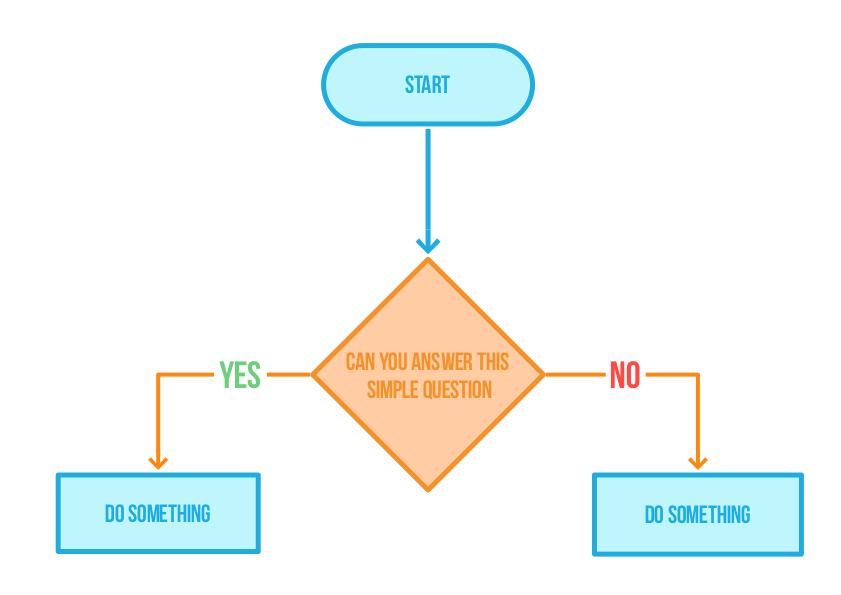
\includegraphics[scale=0.5]{figures/Flowchart}
    \caption{Caption for flowchart}
  	\medskip 
	\hspace*{15pt}\hbox{\scriptsize Credit: Acme company makes everything \url{https://acme.com/}}
    \label{FlowchartFigure}
\end{figure}

\subsection{Tables}

We can also do tables. Protip: use \url{https://www.tablesgenerator.com/} for generating tables.
\begin{table}[H]
\centering
\caption{Caption of table}
\label{TableLabel}
\begin{tabular}{|l|l|l|}
\hline
Title1 & Title2 & Title3 \\ \hline
data1  & data2  & data3  \\ \hline
\end{tabular}
\end{table}

\subsection{\gls{git}}

\gls{git} is fun, use it!

\chapter{Background}
In this chapter, the field of cryptology will be introduced, with an emphasis on digital signatures and cryptanalysis.  
We also introduce some necessary facts and notions related to linear algebra and lattices, as well as probability theory and distributions.
Lastly, we introduce the notion of \textit{Gradient Search} and ADAM-optimizers, which will be a central tool in this thesis.

\section{Cryptology}
For this section, \cite{KL20} will be used.
\subsection{Cryptography}
\subsection{Cryptanalysis}

\section{Digital Signatures}
\subsection{Hash-and-Sign}
\subsection{GGH}
\subsection{NTRU}
\section{Algebra}
\subsection{Polynomials}
\subsection{Polynomial rings}
\subsection{Number fields}
\section{Linear Algebra and Lattices}
Denote by $\vec{v}$ an $n \times 1$ column vector on the form 
\[ \vec{v} = \begin{bmatrix} v_0 \\ v_1 \\ ... \\ v_{n-1} \end{bmatrix}\] and by $\mat{B}$ an $n \times m$ matrix on the form 
\[
    \mat{B} = 
    \begin{bmatrix}
        b_{0,0} & b_{0,1} & \cdots & b_{0, n-1} \\ 
        b_{1,0} & b_{1,1} & \cdots & b_{1, n-1} \\ 
        \cdots & \cdots & \cdots & \cdots\\
        b_{m-1,0} & b_{m-1,1} & \cdots & b_{m-1, n-1} \\ 
    \end{bmatrix}
\]

Generally, entries $v_i$ and $b_{i, j}$ are integers unless stated otherwise.
Some places the thesis will use row notation instead of column notation for the vectors, so that $\vec{v}$ is a $1 \times n$ row vector on the form
\[\vec{c} = [v_0, v_1, ..., v_{n-1}]\] In these cases this will be pointed out.

We denote by $\langle \cdot, \cdot \rangle$ the dot-product of two vectors of equal dimensions as \\
$\langle \vec{x}, \vec{y} \rangle = \vec{x}^t \vec{y} = \mathlarger{\sum_{i=0}^{n-1} x_i y_i}$
\section{Probability Theory}
\section{Gradient Search}

\chapter{Hawk and \textit{Learning a parallelepiped}}

\section{Hawk}
In the following Hawk, the digital signature scheme, will be presented, as in \cite{hawkspec}
\subsection{Simple Hawk}
Present simple sketch of keygen, sign and ver, as well as an example in dimension 2
\subsection{Key generation}
\subsection{Signature generation}
\subsection{Signature verification}

\section{Learning a parallelepiped}
The paper \textit{Learning a Parallelepiped: Cryptanalysis of GGH and NTRU Signatures} by Phong Q. Nguyen and Oded Regev from 2006 \cite{hpp}
introduced a method for breaking signature schemes that follow the GGH structure. By collecting enough signatures on the form $\mathbf{s} = \nint{\textbf{m} \mathbf{B}^{-1}}\mathbf{B}$
where $\mathbf{m}$ is a hash of some message and $\mathbf{B}$ is the secret basis, one can easily recover $\mathbf{B}$. 
\subsection{Assumptions}
First we look at an idealized case to get some understanding of the Hidden Parallelepiped Problem:
Let $\mathbf{B}$ be a secret $n \times n$ matrix. Let $\{\mathbf{s}_1, \mathbf{s}_2, ... \mathbf{s}_p\}$ where $\mathbf{s}_i = \nint{\textbf{m}_i \mathbf{B}^{-1}}\mathbf{B}$
and $\mathbf{m}_i$ is uniformly distributed over some interval $[0, q]$ be $p$ signatures on "random" messages.
\subsection{Covariance matrix}
\subsection{Hidden parallelepiped to hidden hypercube}
\subsection{Gradient descent}
\subsection{Example in dimension 2}
\subsection{Hawk resistance against HPP}

\chapter{Implementation}
Introduction to the implementation part of the thesis
\section{Implementation of Hawk}
Something something about the implementation of Hawk in Rust.
Mentions of sampling, integer/float types, speed and comparison to Hawk team's C code? \hfill \break \\
\section{Implementation of HPP}
Something something about the implementation of HPP in Rust. Something about speedup/parallelization of gradient descent?

\chapter{Adapting HPP to Hawk}
In this chapter we investigate the steps needed to possibly apply the Hidden Parallelepiped Problem to the Hawk digital signature scheme.
\section{Covariance matrix secret key in Hawk}
Nothing yet I'm afraid
\section{Secret Key Recovery}
Since $\mathbf{x}$ follows some distribution close to some normal distribution, we hope that enough vectors $\mathbf{w}$ will disclose some information about $\mathbf{B}^{-1}$.
If we know $\mathbf{B}^{-1}$ we know $\mathbf{B}$. This is the goal.


% Include more chapters as required.
%%=========================================

% Alternative 1 of printing glossaries & acronyms
%\renewcommand{\glossarypreamble}{\footnotesize}
%\printglossary[style=super, type=\glsdefaulttype] \let\cleardoublepage\clearpage
%\printglossary[style=super, type=\acronymtype]


%Alternative 2
%Simplified way of printing glossaries, slower than alt 1, but has better compatibility
% \printnoidxglossaries

% Include more appendices as required.
%%=========================================
\clearpage
\DeclareRobustCommand{\VAN}[3]{#3}
\addcontentsline{toc}{chapter}{Bibliography}
\bibliographystyle{generators/myplainnat}
\bibliography{generators/refs}
\appendix
\titleformat{\chapter}[display]
  {\normalfont\large\bfseries}% <- font for label "Appendix A", default \huge
  {\chaptertitlename\ \thechapter}
  {20pt}
  {\large}% <- font for title, default \Huge

\chapter{Generated code from Protocol buffers}

\begin{lstlisting}[caption={Source code of something},label=Listing]
System.out.println("Hello Mars");
\end{lstlisting}
\end{document}
